% !TeX spellcheck = en_US
\section{Problem 12}

In order to evaluate the expression "\verb|not(A(x) OR B(x))|", we first have to take a look in how fuzzy logic is different with binary logic at the operation level.
In binary logic we have three basic operations: \verb*|AND(x,y)|, \verb*|OR(x,y)| and \verb*|NOT(x)|. But, in fuzzy logic, where a function can have a value in range of $\left[0...1\right]$, things are a bit different.
Operation \verb*|AND(x,y)| of binary is equivalent with \verb|MIN(x,y)| from the fuzzy logic, \verb*|OR(x,y)| with \verb*|MAX(x,y)| and \verb*|NOT(x)| with \verb|1-x|.

\begin{wrapfigure}{R}{0.5\textwidth}
	\centering
	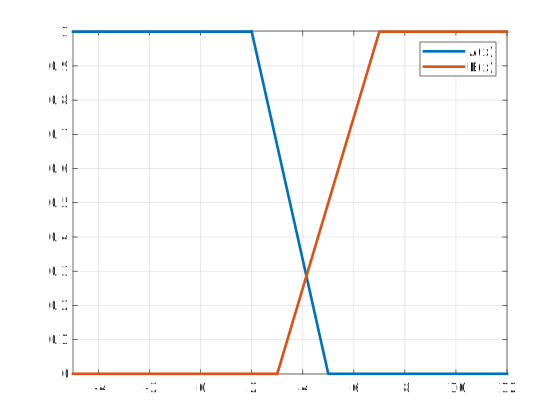
\includegraphics[width=0.4\textwidth]{../Problem 12/a_b_functions.pdf}
	\caption{Plot of A(x), B(x)}
	\label{fig:prob_12_a_b}
\end{wrapfigure}

We have to find the proper $x$ for which the previous expression has the greater value. Firstly, we will calculate the expression and then find the proper $x$.
To achieve this, we will have to break down our calculations in areas. 

Starting with $x \le 2$, $"A(x) \text{ AND } B(x)"$ is equal to $"\max\left(A(x), B(x)\right)" = 1$. So, using De Morgan's law, we have $\textit{max}\left(A(x), B(x)\right) = \textit{not}\left(A(x) \textit{ or } B(x)\right) = 0$.
The exact same result is obtained at $x \ge 7$.

Things are a bit different in $2 \le x \le 7$. Function $A(x)$ starts to fall while $B(x)$ starts to rise. The point where they cross is valuable for defining the expression needed and can be found by solving the equation 
\[
A(x) = B(x) \Leftrightarrow 1 - \frac{x-2}{3} = \frac{x-3}{4} \Rightarrow x = \frac{29}{7}
\]

So, for $2 \le x \le \frac{29}{7}$, $\textit{max}\left(A(x), B(x)\right) = 1 - \dfrac{x-2}{3} = A(x)$, because in this region $A(x)$ is above $B(x)$. Thus, $\textit{not}\left(A(x) \textit{ or } B(x)\right) = \dfrac{x-2}{3}$.

Using the same logic, we find out that for $\frac{29}{7} \le x \le 7$, $\textit{not}\left(A(x) \textit{ or } B(x)\right) = 1 - \dfrac{x-3}{4}$. 

Therefore, the expression $f(x) = \textit{not}\left(A(x) \textit{ or } B(x)\right)$ is summarized in the following:
\begin{equation}
	f(x) = \left\{
	\begin{array}{cc}
		0 & x \le 2, \\[3pt]
		\dfrac{x-2}{3} & 2 \le x \le \frac{29}{7}, \\[7pt]
		1 - \dfrac{x-3}{4} & \frac{29}{7} \le x \le 7, \\[3pt]
		0 & x \ge 7\\
	\end{array}
	\right.
\end{equation}